\pgfplotsset{compat=1.9}

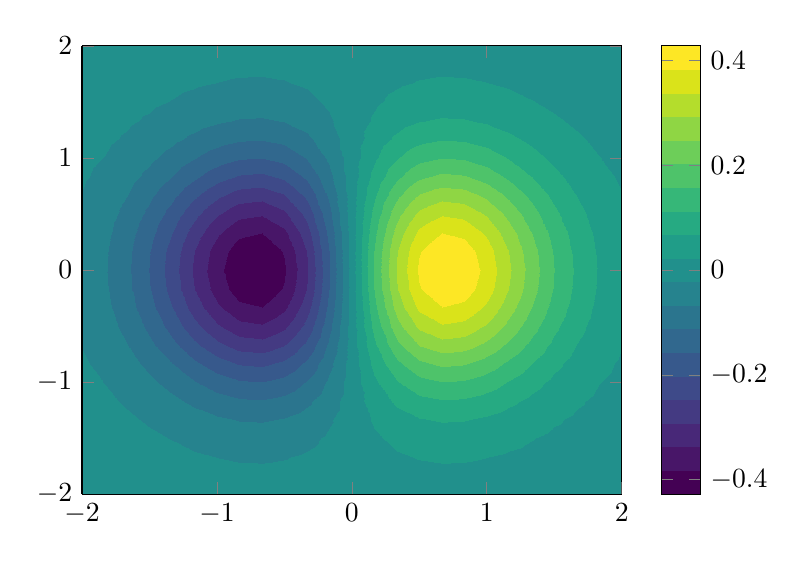
\begin{tikzpicture}
\begin{axis}[
%    title={$x \exp(-x^2-y^2)$},
    domain=-2:2, view={0}{90}, colorbar right, colormap name = viridis ]
    
  \addplot3 [contour filled={number=19,},] 
  {exp(-x^2-y^2)*x};
  
\end{axis}
\end{tikzpicture}

% it looks a bit rough - try tweaking it to look better